% !Mode:: "TeX:UTF-8"

\documentclass[12pt,openany,oneside]{book}

% !Mode:: "TeX:UTF-8"
% !Tex Program = xelatex
% Author: Unlucky(http://blog.thebeyond.name)
%         Myautsai(http://mckelv.in)

%%%%%%%%%% Package %%%%%%%%%%%%
\usepackage{graphicx}                       % 支持插图处理
\usepackage[a4paper,
              text={148true mm,223true mm},
			  top=37true mm,
			  bottom=37true mm,
			  left=31true mm,
			  right=31true mm,
			  head=7true mm,
			  headsep=2.5true mm,
			  foot=7true mm
			]{geometry}                      % 支持版面尺寸设置
\usepackage{titlesec}                       % 控制标题的宏包
\usepackage{titletoc}                       % 控制目录的宏包
\usepackage{fancyhdr}                       % fancyhdr宏包 支持页眉和页脚的相关定义
%\usepackage[UTF8]{ctex}
\usepackage[CJKnumber]{xeCJK}                 %xeCJK中文支持,并提供将阿拉伯数字转换成中文数字的命令
\usepackage{color}                          % 支持彩色
\usepackage{amsmath}                        % AMSLaTeX宏包 用来排出更加漂亮的公式
\usepackage{amssymb}                        % 数学符号生成命令
\usepackage[below]{placeins}                %允许上一个section的浮动图形出现在下一个section的开始部分,还提供\FloatBarrier命令,使所有未处理的浮动图形立即被处理
\usepackage{flafter}                        % 使得所有浮动体不能被放置在其浮动环境之前,以免浮动体在引述它的文本之前出现.
\usepackage{multirow}                       % 使用Multirow宏包,使得表格可以合并多个row格
\usepackage{booktabs}                       % 表格,横的粗线;\specialrule{1pt}{0pt}{0pt}
\usepackage{longtable}                      % 支持跨页的表格。
\usepackage{tabularx}                       % 自动设置表格的列宽
\usepackage{subfigure}                      % 支持子图 %centerlast 设置最后一行是否居中
\usepackage[subfigure]{ccaption}            % 支持子图的中文标题
\usepackage[sort&compress,numbers]{natbib}  % 支持引用缩写的宏包
\usepackage{enumitem}                       % 使用enumitem宏包,改变列表项的格式
\usepackage{calc}                           % 长度可以用+ - * / 进行计算
\usepackage{txfonts}                        % 字体宏包
\usepackage{bm}                             % 处理数学公式中的黑斜体的宏包
\usepackage[amsmath,thmmarks,hyperref]{ntheorem}  % 定理类环境宏包,其中 amsmath 选项用来兼容 AMS LaTeX 的宏包
%\usepackage{CJKnumb}                        % 提供将阿拉伯数字转换成中文数字的命令
\usepackage{indentfirst}                    % 首行缩进宏包
%\usepackage{CJKutf8}                        % 用在UTF8编码环境下,它可以自动调用CJK,同时针对UTF8编码作了设置。
%\usepackage{hypbmsec}                      % 用来控制书签中标题显示内容
\usepackage{CJKfntef}

\usepackage{times}
\usepackage{fontspec,xunicode,xltxtra}      % XeLaTeX相关字体字库

%如果您的pdf制作中文书签有乱码使用如下命令,就可以解决了
\usepackage[xetex, unicode,
              pdfstartview=FitH,
              CJKbookmarks=true,
              bookmarksnumbered=true,
              bookmarksopen=true,
              colorlinks=true,
			  citecolor=black,
              linkcolor=black,
              anchorcolor=black,
              urlcolor=black,
              breaklinks=true
            ]{hyperref}
 % 定义所需宏包

\begin{document}
% !Mode:: "TeX:UTF-8"
% Author: Unlucky(http://blog.thebeyond.name)
%         MCKelvin(http://mckelv.in)

%%%%%%%%%% Fonts Definition and Basics %%%%%%%%%%%%%%%%%
\XeTeXlinebreaklocale "zh"
\XeTeXlinebreakskip = 0pt plus 1pt minus 0.1pt
\setCJKfamilyfont{song}{SimSun}             % 宋体
\newcommand{\song}{\CJKfamily{song}}
\setCJKfamilyfont{fs}{FangSong}             % 仿宋体
\newcommand{\fs}{\CJKfamily{fs}}
\setCJKfamilyfont{kai}{KaiTi}               % 楷体
\newcommand{\kai}{\CJKfamily{kai}}
\setCJKfamilyfont{hei}{SimHei}              % 黑体
\newcommand{\hei}{\CJKfamily{hei}}
\setCJKfamilyfont{li}{LiSu}                 % 隶书
\newcommand{\li}{\CJKfamily{li}}
\setCJKfamilyfont{tnroman}{Times New Roman} % Times New Roman
\newcommand{\tnroman}{\CJKfamily{tnroman}}

\newcommand{\yihao}{\fontsize{26pt}{26pt}\selectfont}       % 一号, 单倍行距
\newcommand{\xiaoyi}{\fontsize{24pt}{24pt}\selectfont}      % 小一, 单倍行距
\newcommand{\erhao}{\fontsize{22pt}{22pt}\selectfont}       % 二号, 单倍行距
\newcommand{\xiaoer}{\fontsize{18pt}{18pt}\selectfont}      % 小二, 单倍行距
\newcommand{\sanhao}{\fontsize{16pt}{16pt}\selectfont}      % 三号, 单倍行距
\newcommand{\xiaosan}{\fontsize{15pt}{22.5pt}\selectfont}   % 小三, 1.5倍行距
\newcommand{\sihao}{\fontsize{14pt}{14pt}\selectfont}       % 四号, 单倍行距
\newcommand{\xiaosi}{\fontsize{12pt}{18pt}\selectfont}      % 小四, 1.5倍行距
\newcommand{\wuhao}{\fontsize{10.5pt}{10.5pt}\selectfont}   % 五号, 单倍行距
\newcommand{\xiaowu}{\fontsize{9pt}{9pt}\selectfont}        % 小五, 单倍行距

\setmainfont{Times New Roman}
\setCJKmainfont{SimSun}
\setCJKmonofont{SimSun}

% \CJKcaption{gb_452}
% \CJKtilde  % 重新定义了波浪符~的意义
\newcommand\prechaptername{第}
\newcommand\postchaptername{章}

% \punctstyle{plain}
% 调整罗列环境的布局
\setitemize{leftmargin=3em,itemsep=0em,partopsep=0em,parsep=0em,topsep=-0em}
\setenumerate{leftmargin=3em,itemsep=0em,partopsep=0em,parsep=0em,topsep=0em}
% \setlength{\baselineskip}{20pt}
% \renewcommand{\baselinestretch}{1.38} % 设置行距

% 避免宏包 hyperref 和 arydshln 不兼容带来的目录链接失效的问题。
\def\temp{\relax}
\let\temp\addcontentsline
\gdef\addcontentsline{\phantomsection\temp}

% 自定义项目列表标签及格式 \begin{publist} 列表项 \end{publist}
\newcounter{pubctr} %自定义新计数器
\newenvironment{publist}{%%%%%定义新环境
  \begin{list}{[\arabic{pubctr}]} %%标签格式
    {
      \usecounter{pubctr}
      \setlength{\leftmargin}{2.5em}   % 左边界 \leftmargin =\itemindent + \labelwidth + \labelsep
      \setlength{\itemindent}{0em}     % 标号缩进量
      \setlength{\labelsep}{1em}       % 标号和列表项之间的距离,默认0.5em
      \setlength{\rightmargin}{0em}    % 右边界
      \setlength{\topsep}{0ex}         % 列表到上下文的垂直距离
      \setlength{\parsep}{0ex}         % 段落间距
      \setlength{\itemsep}{0ex}        % 标签间距
      \setlength{\listparindent}{0pt}  % 段落缩进量
    }}
  {\end{list}}%%%%%

\makeatletter
\renewcommand\normalsize{
  \@setfontsize\normalsize{12pt}{18pt} % 小四对应12pt,1.5倍行距对应18pt
  \setlength\abovedisplayskip{4pt}
  \setlength\abovedisplayshortskip{4pt}
  \setlength\belowdisplayskip{\abovedisplayskip}
  \setlength\belowdisplayshortskip{\abovedisplayshortskip}
  \let\@listi\@listI}
\def\defaultfont{\renewcommand{\baselinestretch}{1.35}\normalsize\selectfont} %Word和XeLaTeX行距的缩放因子,Word偏小,该值为实验值,可根据实际情况做修改
% 设置行距和段落间垂直距离
\renewcommand{\CJKglue}{\hskip 0.96pt plus 0.08\baselineskip} %加大字间距,使每行33个字

\makeatother
%%%%%%%%%%%%% Contents %%%%%%%%%%%%%%%%%
% 主目录设置
\renewcommand{\contentsname}{目\qquad 录}
\setcounter{tocdepth}{1}
% Chapter目录设置
\titlecontents{chapter}[2em]{\vspace{.5\baselineskip}\wuhao\hei}
{\prechaptername\CJKnumber{\thecontentslabel}\postchaptername\qquad}{}
{\hspace{.5em}\titlerule*[10pt]{$\cdot$}\wuhao\contentspage}
% Section目录设置
\titlecontents{section}[3em]{\vspace{.25\baselineskip}\wuhao\song}
{\thecontentslabel\quad}{}
{\hspace{.5em}\titlerule*[10pt]{$\cdot$}\wuhao\contentspage}
% Subsection目录设置
\titlecontents{subsection}[4em]{\vspace{.25\baselineskip}\wuhao\song}
{\thecontentslabel\quad}{}
{\hspace{.5em}\titlerule*[10pt]{$\cdot$}\wuhao\contentspage}

% 图目录设置
\renewcommand{\listfigurename}{图目录}
\newcommand{\loflabel}{图}
\renewcommand{\numberline}[1]{\loflabel~#1\hspace*{1em}}

% 表目录设置
\renewcommand{\listtablename}{表目录}
\newcommand{\lotlabel}{表}
\renewcommand{\numberline}[1]{\lotlabel~#1\hspace*{1em}}


%%%%%%%%%% Chapter and Section %%%%%%%%%%%%%%%%%
\setcounter{secnumdepth}{4}
\setlength{\parindent}{2em}
\renewcommand{\chaptername}{\prechaptername\CJKnumber{\thechapter}\postchaptername}
\titleformat{\chapter}{\centering\hei\xiaoer\bfseries}{\chaptername}{2em}{}
\titlespacing{\chapter}{0pt}{0.3\baselineskip}{1\baselineskip}
\titleformat{\section}{\hei\xiaosan\bfseries}{\thesection}{1em}{}
\titlespacing{\section}{0pt}{0.2\baselineskip}{0.5\baselineskip}
\titleformat{\subsection}{\hei\sihao\bfseries}{\thesubsection}{1em}{}
\titlespacing{\subsection}{0pt}{0.1\baselineskip}{0.3\baselineskip}
\titleformat{\subsubsection}{\xiaosan\bfseries}{\thesubsubsection}{1em}{}
\titlespacing{\subsubsection}{0pt}{0}{0}

%%%%%%%%%% Table, Figure and Equation %%%%%%%%%%%%%%%%%
\renewcommand{\tablename}{表} % 插表题头
\renewcommand{\figurename}{图} % 插图题头
\renewcommand{\thefigure}{\arabic{chapter}-\arabic{figure}} % 使图编号为 7-1 的格式 %\protect{~}
\renewcommand{\thesubfigure}{\alph{subfigure})}%使子图编号为 a)的格式
\renewcommand{\thesubtable}{(\alph{subtable})} %使子表编号为 a)的格式
\renewcommand{\thetable}{\arabic{chapter}-\arabic{table}}%使表编号为 7-1 的格式
\renewcommand{\theequation}{\arabic{chapter}-\arabic{equation}}%使公式编号为 7-1 的格式

%% 定制浮动图形和表格标题样式
\makeatletter
\long\def\@makecaption#1#2{%
  \vskip\abovecaptionskip
  \sbox\@tempboxa{\centering\wuhao\song{#1\qquad #2} }%
  \ifdim \wd\@tempboxa >\hsize
  \centering\wuhao\song{#1\qquad #2} \par
  \else
  \global \@minipagefalse
  \hb@xt@\hsize{\hfil\box\@tempboxa\hfil}%
  \fi
  \vskip\belowcaptionskip}
\makeatother
\captiondelim{~~~~} %用来控制longtable表头分隔符

%%%%%%%%%% Theorem Environment %%%%%%%%%%%%%%%%%
\theoremstyle{plain}
\theorembodyfont{\song\rmfamily}
\theoremheaderfont{\hei\rmfamily}
\newtheorem{theorem}{定理~}[chapter]
\newtheorem{lemma}{引理~}[chapter]
\newtheorem{axiom}{公理~}[chapter]
\newtheorem{proposition}{命题~}[chapter]
\newtheorem{corollary}{推论~}[chapter]
\newtheorem{definition}{定义~}[chapter]
\newtheorem{conjecture}{猜想~}[chapter]
\newtheorem{example}{例~}[chapter]
\newtheorem{remark}{注~}[chapter]
\newtheorem{algorithm}{算法~}[chapter]
\newenvironment{proof}{\noindent{\hei 证明:}}{\hfill $ \square $ \vskip 4mm}
\theoremsymbol{$\square$}

%%%%%%%%%% Page: number, header and footer  %%%%%%%%%%%%%%%%%

% \frontmatter 或 \pagenumbering{roman}
% \mainmatter 或 \pagenumbering{arabic}
\makeatletter
\renewcommand\frontmatter{\clearpage
  \@mainmatterfalse
  \pagenumbering{Roman}} % 正文前罗马字体编号
\makeatother


%%%%%%%%%% References %%%%%%%%%%%%%%%%%
\renewcommand{\bibname}{参考文献}
% 重定义参考文献样式,来自thu
\makeatletter
\renewenvironment{thebibliography}[1]{%
  \titleformat{\chapter}{\raggedright\sihao\hei}{\chaptername}{2em}{}
  \chapter*{\bibname}%
  \wuhao
  \list{\@biblabel{\@arabic\c@enumiv}}%
  {\renewcommand{\makelabel}[1]{##1\hfill}
    \settowidth\labelwidth{0.5cm}
    \setlength{\labelsep}{0pt}
    \setlength{\itemindent}{0pt}
    \setlength{\leftmargin}{\labelwidth+\labelsep}
    \addtolength{\itemsep}{-0.7em}
    \usecounter{enumiv}%
    \let\p@enumiv\@empty
    \renewcommand\theenumiv{\@arabic\c@enumiv}}%
  \sloppy\frenchspacing
  \clubpenalty4000%
  \@clubpenalty \clubpenalty
  \widowpenalty4000%
  \interlinepenalty4000%
  \sfcode`\.\@m}
{\def\@noitemerr
  {\@latex@warning{Empty `thebibliography' environment}}%
  \endlist\frenchspacing}
\makeatother

\addtolength{\bibsep}{-0.5em} % 缩小参考文献间的垂直间距
\setlength{\bibhang}{2em} %每个条目自第二行起缩进的距离

% 参考文献引用作为上标出现
% \newcommand{\citeup}[1]{\textsuperscript{\cite{#1}}}
\makeatletter
\def\@cite#1#2{\textsuperscript{[{#1\if@tempswa , #2\fi}]}}
\makeatother
%% 引用格式
\bibpunct{[}{]}{,}{s}{}{,}

%%%%%%%%%% Cover %%%%%%%%%%%%%%%%%
% 封面、摘要、版权、致谢格式定义
\makeatletter
\def\ctitle#1{\def\@ctitle{#1}}\def\@ctitle{}
\def\caffil#1{\def\@caffil{#1}}\def\@caffil{}
\def\csubject#1{\def\@csubject{#1}}\def\@csubject{}
\def\cauthor#1{\def\@cauthor{#1}}\def\@cauthor{}
\def\csupervisor#1{\def\@csupervisor{#1}}\def\@csupervisor{}
\def\cdate#1{\def\@cdate{#1}}\def\@cdate{}
\long\def\cabstract#1{\long\def\@cabstract{#1}}\long\def\@cabstract{}
\long\def\eabstract#1{\long\def\@eabstract{#1}}\long\def\@eabstract{}
\def\ckeywords#1{\def\@ckeywords{#1}}\def\@ckeywords{}
\def\ekeywords#1{\def\@ekeywords{#1}}\def\@ekeywords{}
\def\cheading#1{\def\@cheading{#1}}\def\@cheading{}

% 在book文件类别下,\leftmark自动存录各章之章名,\rightmark记录节标题
\pagestyle{fancy}
% 去掉章节标题中的数字 务必放到\pagestyle{fancy}之后才会起作用
%% 不要注销这一行,否则页眉会变成:“第1章1  绪论”样式
\renewcommand{\chaptermark}[1]{\markboth{\chaptername~\ #1}{}}
\fancyhf{}
% \fancyhead[C]{\song\wuhao \leftmark} % 页眉显示章节名称
\fancyhead[C]{\song\xiaowu \@cheading}
% \fancyhead[CO]{\song\wuhao \@cheading}
% \fancyhead[CE]{\song\wuhao \@cheading}
\fancyfoot[C]{\song\xiaowu ~\thepage~}

\fancypagestyle{plain}{% 设置开章页页眉页脚风格
  \fancyhf{}%
  % \fancyhead[C]{\song\wuhao \leftmark}
  \fancyhead[C]{\song\xiaowu \@cheading}
  \fancyfoot[C]{\song\xiaowu ~\thepage~ } %%首页页脚格式
  \renewcommand{\headrulewidth}{0.5pt}%
  \renewcommand{\footrulewidth}{0pt}%
}

% 定义封面
\def\makecover{
  % \cleardoublepage%
  \phantomsection
  \pdfbookmark[-1]{\@ctitle}{ctitle}

  \begin{titlepage}
  	\vspace*{-2.5mm}
    \begin{center}
      %校名
      \begin{figure}[h]
        \centering
        
\includegraphics[width=9.84cm]{figures/zjut}
      \end{figure}
      \vspace*{9.66mm}
	  \song\yihao{本科毕业设计说明书(论文)}\\
	  \vspace*{10.0mm}
	  \hei\xiaoer{(2013届)}\\
      \vspace*{8.5mm}
      %校徽
      \begin{figure}[h]
        \centering
        
\includegraphics[width=2.73cm]{figures/zjutlogo}
      \end{figure}
      \vspace*{0.0mm}
      \renewcommand{\arraystretch}{1.0}
      \begin{tabular}{lc}
        \song\erhao{论文题目\quad} & \song\xiaoer{\@ctitle} \\ \cline{2-2}
      \end{tabular}\\
	  \vspace*{11.1mm}
      \setlength{\arrayrulewidth}{0.5pt}
      {\song\sihao
        \renewcommand{\arraystretch}{2.0}
        \begin{tabular}{lc}
          作者姓名\qquad &  \@cauthor \\ \cline{2-2}
          指导教师\qquad &  \@csupervisor \\ \cline{2-2}
          \\
          学科(专业)\qquad &  \@csubject \\ \cline{2-2}
          所在学院\qquad &  \@caffil \\ \cline{2-2}\cline{2-2}
          提交日期\qquad & \@cdate \\ \cline{2-2}
        \end{tabular}
	  }
    \end{center}
  \end{titlepage}

  %%%%%%%%%%%%%%%%%%% Abstract and Keywords  %%%%%%%%%%%%%%%%%%%%%%%
  \clearpage
  \markboth{摘~要}{摘~要}
  \addcontentsline{toc}{chapter}{摘~要}
  \setlength{\parskip}{24pt}
  \chapter*{\centering\hei\xiaoer{摘\qquad 要}}
  \setlength{\parskip}{18pt}
  \setcounter{page}{1}
  %\song\defaultfont
  \setlength{\parskip}{0pt}
  \song\xiaosi{\@cabstract}
  \vspace{15pt}

  \hangafter=1\hangindent=52.3pt\noindent
  \hei\xiaosi{关键词:} \song\xiaosi{\@ckeywords}

  %%%%%%%%%%%%%%%%%%% English Abstract  %%%%%%%%%%%%%%%%%%%%%%%%%%%%%%
  \clearpage
  % \phantomsection
  \markboth{ABSTRACT}{ABSTRACT}
  \addcontentsline{toc}{chapter}{ABSTRACT}
  \setlength{\parskip}{24pt}
  \chapter*{\centering\tnroman\xiaoer\textbf{ABSTRACT}}
  \setlength{\parskip}{18pt}
  % \vspace{\baselineskip}
  \setlength{\parskip}{0pt}
  \@eabstract
  \vspace{15pt}

  \hangafter=1\hangindent=60pt\noindent
  {\tnroman\xiaosi\textbf{Keywords:}}  {\tnroman\xiaosi{\@ekeywords}}
}
\makeatother  % 格式设置
% !Mode:: "TeX:UTF-8"
%%============================================================
%% 中文封面
\thispagestyle{empty}
\pdfbookmark[-1]{\zjuttitlec}{zjutreportcover}
\phantomsection \label{zjutreportcover}
\vspace*{-2.5mm}
% 校名
\begin{center}
   
\includegraphics[width=98.40mm]{figures/zjut}
\end{center}
\vspace*{9.66mm}
\centerline{\songti\yihao{\reporttitle}}
\vspace*{10.0mm}
\centerline{\heiti\xiaoer\textbf{(\zjutgrade\ 届)}}
\vspace*{8.5mm}
% 校徽
\begin{center}
  
\includegraphics[width=27.3mm]{figures/zjutlogo}
\end{center}

\vspace*{0.0mm}
\renewcommand{\arraystretch}{1.0}
\hspace*{7.4mm}
{\songti\erhao{论文题目}}
\hspace{6mm}
\begin{minipage}[t]{95mm}
    \linespread{1.1}{\songti\xiaoer\uline{\zjuttitlec}}
\end{minipage}
\vspace*{9mm}
\begin{center}
    \setlength{\arrayrulewidth}{0.5pt}
    {\songti\sihao
        \renewcommand{\arraystretch}{1.4}
        \begin{tabular}{lc}
            作者姓名 \qquad &  \zjutauthornamec \\ \cline{2-2}
            指导教师\qquad &  \zjutmentorc\\ \cline{2-2}
            \\
            学科(专业)\qquad &  \zjutmajor \\ \cline{2-2}
            所在学院\qquad &  \zjutcollegec \\ \cline{2-2}\cline{2-2}
            提交日期\qquad & \zjutsubmitteddatee \\ \cline{2-2}
        \end{tabular}
    }
\end{center}

  % 封面

\mainmatter\defaultfont\sloppy\raggedbottom

\begingroup % 在组内的chapter不换行
\let\clearpage\relax % chapter之后不换页
%%%%%%%%%% 摘要 %%%%%%%%%%
\titleformat{\chapter}{\centering\hei\sanhao\bfseries}{\chaptername}{1em}{} % 标题居中,黑体三号
%%%%% 标题 %%%%%
\chapter*{浙江工业大学本科生毕业设计开题报告模板}
\titleformat{\chapter}{\hei\sihao\bfseries}{\chaptername}{1em}{} % 恢复标题居左,黑体四号

%%%%%%%%%% 正文 %%%%%%%%%%
% !Mode:: "TeX:UTF-8"

\chapter{选题的背景与意义}
\section{研究开发的目的}
随着教育部教学质量与教学改革工程建设工作的展开,浙江省教育厅也设立了一批相应的教学质量与教学改革项目。在省级项目立项、国家级项目推荐、已经立项的各类项目的管理与检查等方面,目前浙江省教育厅高等教育处没有相应的电子化的项目管理、项目申报评审系统。为提高管理水平和效率,迫切需要建设项目管理的硬件平台和设计开发一套符合我省教学质量工程项目实际需要的软件系统。建设“浙江省教育厅教学质量与教学改革项目申报管理系统”(暂名,以下简称项目申报管理系统)将能有效地促进高等教育处的管理工作。

(1) 提高管理的质量与效率。\par
目前的高教处的项目管理工作基本上都是基于传统的纸质材料,已经严重落后于电子政务建设的步伐,管理者很难全面地了解把握各类建设项目的立项、建设进展等情况。申报管理系统建设后,将能提供快速、准确、全面的种类项目的立项与建设情况。

(2) 实现项目的网上申报、网上评审。\par
国家教学质量与教学改革工程项目的立项都已经实行网上申报、网上评审,各类科技项目一般也都已经实行网上申报、网上评审。我省教学质量工程项目的申报与评审仍然是传统的纸质材料文件方式。这样既不符合申报材料电子化的趋势,也限制了项目评审专家的选择、项目评审的公平、公正。实行项目的网上申报、网上评审,将大大提高项目评审工作的效率与评审专家的选择范围。

(3) 展示教学质量与教学改革成果,发挥示范作用。\par
在现在基于纸质材料的管理体制下,建设与改革项目的成果难以进行比较大面积的宣传与交流。在拟建设的系统中,设立成果展示平台,发挥优秀成果的示范作用。

\section{国内外研究发展现状}
在国外,教学质量管理已有90年的历史。以美国为代表的许多国家,如澳大 利亚、英国、加拿大、比利时等国都相继采用学生评教来评价教师的教学效果。以美国为例,20世纪70年代初,美国教育委员会的一个调查结果表明,在被调查的669所高等学校中,大约有65%的高校在系一级机构中允许学生对教学进行评价,到80年代以后,学生评教不但成为大学教学评价的二个重要组成部分,且评价技术越来越现代化。目前,许多大学已经开发使用了基于网络的学生评教系统,如华盛顿大学的IAS(Instructional Assessment System)、亚利桑那大学的TCE(Teacher-Course Evaluation)、堪萨斯州立大学的IDEA(Individual Development and Educational Assessment)等[2],这些系统通过校园网络实施教学评价,取得了较好的效果。美国等国家已经有网上申报、网上专家评审的系统,基于网络的申报管理信息系统国外已进入实用研究阶段,大量的投入到各种项目的网上申报、网上评审的实际运用中,提高的项目申报申批的效率,取得了重大的经济效益。

在我国,学生评教的发展经历了定性评教为主和定量评教为主等阶段,比较规范的科学的学生评教活动应当说是伴随科学的高教评估活动的兴起而逐步形成并得到良好发展的。1985年之后开展的各种高教评估试点活动,都离不开对教学质量特别是课堂教学质量的评估,对于后者除了用统测的办法之外,另一个更为可行的办法就是学生评教。我国的学生评教活动始于20世纪80年代初,特别是从1987年起,随着教师职称评定工作日益规范化,许多高校对教师的教学提出了越来越高的要求,学生评教活动开展得越来越普遍。2001年教育部4号文件——《关于加强高等学校本科教学工作提高教学质量的若干意见》出台后,学生评教在全国普通高校更是得到了广泛的开展,评教方式和技术手段也逐步得到了改进。各种基于网络的学生评教信息系统也取得了较大的进展。但相比于国外而言,我国的教学质量网上管理系统的开发还有一定的距离,而且在国家与省级之间也存在着一定的差距。国家教学质量与教学改革工程项目的立项都已经实现网上申报、网上评审,种类科技项目一般也都已经实行网上申报、网上评审。但浙江省高教处的项目管理工作基本上都是基于传统的纸质材料,已经严重落后于电子政务建设的步伐,管理很难全面地了解把握各类建设项目的立项、建设进展等情况。这样既不符合申报材料电子化的趋势,也限制了项目评审专家的选择、项目评审的公平、公正。因此,在国外已进入实用研究阶段时,国内还处于设想开发的初级阶段。

% !Mode:: "TeX:UTF-8"

\chapter{研究开发的基本内容、目标,拟解决的主要问题或技术关键}
\section{研究目标}
在对比国内外教学质量工程申报评审系统的基本上,在研究国外内类似系统的设计实现上,提出自己的设计与实现。在当前教育优先发展的情况下,国家实施科教兴国战略,在这种情况下,教学质量当然也是非常重要的一个因素,关于如何提高教学质量,国家和学校都做了一些探索。特别在当信息技术如此普及的时代,借助信息技术来提高教学质量已是一种普遍的做法,国外已经在这方面走在了前头。本课题的研究目标定位于利用J2EE技术来实现教学质量工程申报评审系统的实现,特别是应用J2EE中的一些关键技术和框架,如Hibernate、Spring、Spring MVC。

\section{研究的基本内容}
由于整个系统的结构庞大,开发工作量大,所以本研究的基本内容并不定位于整个系统的设计与实现上。相反,本研究的基本内容是教学质量工程申报评审系统中的申报子系统功能模块上。
申报子系统的主要功能是根据教育厅发布的项目申报指南和限额,项目申报单位(学校)组织本校教师集中进行项目的申报及对项目的初审。
本研究的具体容包括:

(1)	信息发布\par
信息发布的主要功能是申报通知、申报指南等信息发布,主要是文字内容和相关文档附件。发布信息只能由教育厅主管部门人员进行。对于撰写完毕的信息,可以存入草稿箱中,等待用户修改后发布。对信息提供添加、删除、修改功能。

(2)	项目申报\par
项目申报的主要功能是项目申报人根据学校分发的项目申报密钥进行项目申报书的填写。申报项目的类型和项目的名称已由学校事先录入,申报人不得更改。申报人需要填写在线项目申报简表,上传项目申报书(PDF格式)。填写中可对内容保存、提供修改功能。最后,把申报简表和申报书一起提交到学校。

项目的申报是项目申报子系统中的一个重要的功能,也是该子系统的核心功能。主要包括两大模块填写申报书和提交申报书。

申报人必须按规定在线填写申报简表,按申报书要求离线填写项目申报书,然后把申报简表和项目申报书提交学校。项目的名称和类别已经由学校指定,申报人不得修改;如需修改,必须由学校进行修改。
项目申报信息的填写可以中途保存或填写完毕后提交。提交的申报项目将不能修改。在项目申报的有效时间段内,用户都可以凭密钥登陆系统。项目申报书提交后就不能修改,但可查阅。系统不设置自动提交项目申报材料功能,提交工作由申报人手工操作,并进行确认。

申报简表和申报书核对无误后,申报人把申报简表和项目申报书提交到学校。项目申报书提交后就不能修改,若要修改,需要由学校先进行退回操作。

(3)	学校申报管理\par
各申报单位(学校)负责管理本单位的项目申报工作,并对项目进行初审。学校根据教育厅下达的种类项目的申报限额和申报截止时间,建立本校的具体申报项目和相应的用户密钥,完成本校申报项目的初审并报送教育厅。若申报时间逾期,学校将不能向教育厅提交项目申报,除非教育厅给予再次授权开通。学校在向教育厅正式提交项目申报前,可对申报人所提交的申报材料进行查阅、审核,可以把申报材料退回申报人进行修改,但当正式提交教育厅后,就不能再对申报材料进行修改操作。

在申报系统中,每个学校只能查看本校申报的项目。

新建申报项目。学校在教育厅所授权指定的项目类型中进行项目申报的新建。新建的申报项目数量不得超过教育厅设定的本校申报限额。新建申报项目需要指定项目的名称、项目所属的学科门类(便于项目分组和专家匹配)和指定申报用户密钥。对新建项目申报以列表形式显示,并标示为待填报状态。列表显示新建申报项目的公共属性(如项目类型、项目所属学科门类、项目申报人、用户名)。教师申报用户凭学校分发的密钥进行项目申报书的填写。申报系统对列表中的新建申报项目,提供查看、修改、删除操作。

待初审项目。在申报用户提交后,项目即转入等初审状态。学校对申报项目进行初审,对需要修改的申报项目,可以退回申报人进行修改。

初审通过项目。对初审通过的项目,标示状态为初审通过。对初审通过的项目,提供同类别申报项目的整批提交操作。系统不提供逐个项目单独提交的功能。系统提供对初审项目的优先排序等特殊标记功能。
已提交项目。向教育厅提交的本校申报项目。对已经提交的项目标示已提交教育厅的状态。对项目的提交,只允许提交一次,且前提条件为提交项目的总数不得超过限额,对于小于限额数量的提交操作,给出提醒信息。若一次提交了部分项目,之后又要再提交一些项目,则需要管理员将已经提交的项目退回,申报单位一次性提交全部项目。

(4)	申报设定\par
申报设定的主要功能是对项目申报类别和每个类别各学校相应申报数量的管理。只有启用的申报类别,在学校申报管理中出现。同时可以启用多个申报类别。设定每个申报类别的申报评审时间限制。

\section{需要解决的技术难点}
Spring MVC,Hibernate,Spring框架的整合使用。\par
Ajax技术的使用。\par
密钥的生成与管理。\par

% !Mode:: "TeX:UTF-8"

\chapter{系统实现技术方法研究}
信息管理系统的实现技术多种多样,所以选择合理的技术来实现系统也是一个重大的环节,如果所选择的技术不当,将对系统的实现造成一定的麻烦,可能还会影响系统的性能。J2EE[7]是实现信息管理系统的一种有效技术,当前用J2EE实现B/S结构的信息管理系统非常的流行且技术也越来越趋于成熟,性能也得到了非常大的提升。轻量级的J2EE应用对于小中型项目的开发带来了许多便利之处,对比于经典J2EE的简化,在保留经典J2EE应用的框架、良好的可扩展性、可维护性的基础上,简化了J2EE应用的开发,降低了J2EE应用的部署成本,基本实现过程简明了。轻量级J2EE应用面向的是用户,是一种更实际的信息化平台架构。

基于Web的J2EE Framework在J2EE的世界内已是空前繁荣,几乎每隔一两个星期就会有新的MVC框架发布。目前比较好的框架中有老牌的Struts、WebWork;新兴的有Spring MVC[9]、Tapestry、JSF等。这些大多是著名团队的作品,另外还有一些边缘团队的作品,也相当出色,如Dinamica、VRaptor等。这些框架都提供了较好的层次分隔能力。在实现良好的MVC分隔的基础上,通过提供一些现成的辅助类库,同时也促进了生产效率的提高。而如何选择一个好的框架应用在项目中,将会对项目的效率与可重用生成重大影响。

实现轻量级J2EE的Spring、Hibernate框架是在各种流行框架之中脱颖而出,逐渐成为软件开发人才,特别是WEB程序开发人才喜爱的开发技术。

本系统的开发拟采用Spring(Spring MVC)、Hibernate框架。以下是框架的简单特征与其在系统开发中的作用。

\section{Spring框架}
服务层的著名开发框架Spring[16]本身就是基于MVC结构的,此外它还具有一些良好的特性,如IOC(或DI)和AOP。Inversion of Control(IOC) 控制反转,就是程序的主控权由应用程序代码本身转移到了框架或容器。Dependency Injection(DI)依赖注入,是一个更能描述其特点的名字,可以解释为容器在运行期将某种依赖关系注入到组件中。

Aspect-Oriented Programming(AOP)面向方面编程通过提供另一种考虑程序结构的方式来补充面向对象编程(OOP)。面向对象将应用程序分解成各个层次的对象,而AOP将程序分解成各个方面或者说关注点。这种方式能够模块化例如事务管理这种横切多个对象的关注点(这种关注点术语称作横切关注点)。AOP框架是Spring的一个关键组件,但Spring IOC容器(Bean Factory)和(Application Context)并不依赖于AOP ,这就意味着如果不需要使用AOP则可不用。AOP补充了Spring IOC ,以提供一个有效的中间件解决方案。[21]

Spring的精简项目的代码量方面做出了非常出色的工作,将大量需要重复书写的代码提取出来,进行切面编程。配置文件的灵活性也使项目的灵活性得到的加强,可以在不改变代码的情况下,而只有改变其中的配置文件实现整个系统的改变。

\section{Spring框架的MVC实现[17]——Spring MVC}
Spring的WEB框架是围绕DispatcherServlet来进行设计的。DispatcherServlet的作用是将请求分发到不同的处理器。图~\ref{fig:req_proc}~展示了DispatcherServlet对请求的处理流程。
\begin{figure}[htbp]
\centering
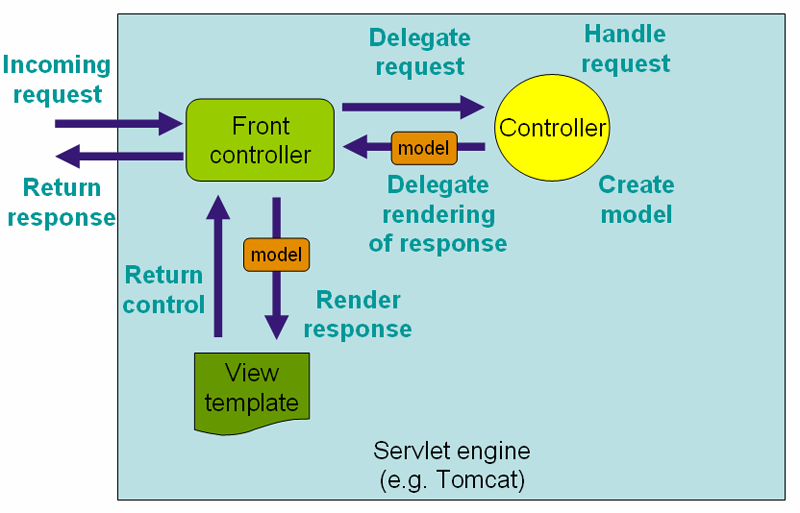
\includegraphics[width=11.65cm]{req_proc}
\caption{Spring Web MVC处理请求工作流程}\label{fig:req_proc}
\vspace{\baselineskip}
\end{figure}
\begin{table}[htbp]
\caption{WebApplicationContext中特殊的bean}\label{tab:bean}
\vspace{0.5em}\centering\wuhao
\begin{tabular}{|m{6cm}|m{6cm}|}
\toprule[1.5pt]
名称 & 描述\\
\midrule[1pt]
控制器(Controller) & 控制器实现的是MVC中Controller那部分\\ \hline
处理器映射(Handler mapping) & 处理器映射包含预处理器(pre-processor),后处理器(post-processor)和控制器的列表,它们在符合某种条件时才被执行(例如符合控制器指定的URL)\\ \hline
视图解析器(View resolvers) & 视图解析器 可以将视图名解析为对应的视图\\ \hline
本地化解析器(Locale resolver) & 本地化解析器能够解析用户正在使用的本地化配置,以提供国际化视图\\ \hline
主题解析器(Theme resolver) & 主题解析器能够解析你的web应用所使用的主题,以提供个性化的布局\\ \hline
上传文件解析器(multipart file resolver) & 上传文件解析器提供HTML表彰文件上传功能\\ \hline
处理异常解析器(Handler exception resolver(s)) & 处理器异常解析器可以将异常对应到视图,或者实现更加复杂的异常处理代码\\
\bottomrule[1.5pt]
\end{tabular}
\vspace{\baselineskip}
\end{table}
DispatcherServlet实际上是一个Servlet,它从HttpServlet继承而来。和其它Servlet一样,DispatcherServlet定义在web应用的web.xml文件中。Spring的Dispatcher有一组特殊的bean,如表~\ref{tab:bean}~所示,用来处理请求和渲染相应的视图。

\section{Hibernate框架}
Hibernate[18]是一种Java语言下的对象关系映射解决方案,它是一种自由、开源的软件。它用来把对象模型表示的对象映射到基于SQL的关系模型结构中去,为面向对象的领域模型到传统的关系型数据库的映射,提供了一个使用方便的框架。Hibernate不仅管理Java类到数据库表的映射(包括从Java数据类型到SQL数据类型的映射),还提供数据查询和获取数据的方法,可以大幅度减少开发时人工使用SQL和JDBC处理数据的时间。它的设计目标是将软件开发人员从大量相同的数据持久层相关编程工作中解放出来。无论是从设计草案还是从一个遗留数据库开始,开发人员都可以采用Hibernate。

下面从Hibernate的体系结构与Hibernate API两方面对Hibernate进行介绍。

(1) hibernate体系结构简介
\begin{figure}[htbp]
\centering
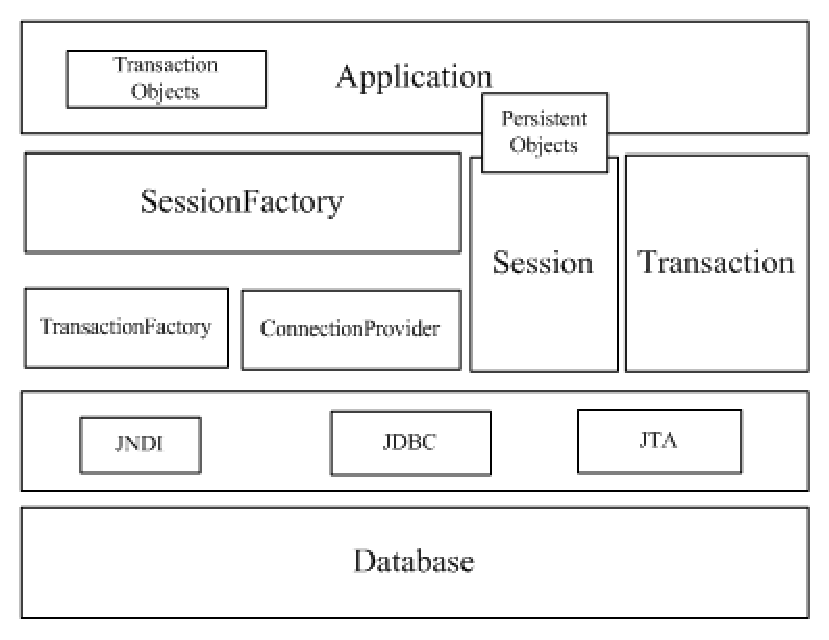
\includegraphics[width=10.01cm]{arch}
\caption{Hibernate体系结构图}\label{fig:arch}
\vspace{\baselineskip}
\end{figure}
图~\ref{fig:arch}~各对象的说明如下:\par
SessionFactory:针对单个数据库映射关系经过编译后的内在镜像,是线程安全的,它是生成Session的工厂。\par
Session:表示应用程序与持久存储层之间交互操作的一个单纯种对象,此对象生存期很短。其隐藏了JDBC连接,也是Transaction的工厂。\par
持久对象及集合:带有持久化状态的、具有业务功能的单线程对象,此对象生存期很短。这些对象可能是普通的JavaBeans/POJO,唯一特殊的是他们正与(仅仅一个)Session相关联。一旦这个Session被关闭,这些对象就会脱离持久化状态,这样就可被应用程序的任何层自由使用。\par
瞬态(transient)和脱管(detached)的对象及其集合:那些目前没有与session关联的持久化类实例。他们可能是在被应用程序实例化后,尚未进行持久化的对象,也可能是因为实例化他们的Session已经被关闭而脱离持久化的对象。\par
事务Transaction:应用程序用来指定原子操作单元范围的对象,它是单线程了,生命周期很短。\par
Hibernate作为模型/数据访问层。它通过配置文件(hiberante.cfg.xml或hibernate.properties和映射文件(*.hbm.xml)把java对象或持久化对象(Persistent Obeject,PO)映射到数据库中的数据表,然后通过操作PO,对数据库中的表进行各种操作。

(2) Hibernate API简介\par
Hibernate API中的接口可分为以下几类:\par
(a)	提供访问数据库的操作的接口,包括Session、Transaction、Query接口。\par
(b)	用于配置Hibernate的接口,Configuration(如下在Spring应用中,将由Spring来完成Hibernate的相关配置)。\par
(c)	间接接口,使应用程序接受Hibernate内部发生的事件,并作出相应的回应,包括:Interceptor、LifeCycle、Validatable。\par
(d)	用户于扩展Hibernate功能的接口,如UserType、CompositeUserType接口。\par
Hibernate内部还封装了JDBC、JTA(Java Transaction API)和JNDI(Java Naming And Directory Interface)。其中,JDBC提供底层的数据访问操作,只要用户提供了相应的JDBC驱动程序,Hibernate可以访问任何一个数据库系统。JTA和JNDI使Hibernate能够和J2EE应用服务器集成。具体接口间的协作如图~\ref{fig:interface}~所示。 
\begin{figure}[htbp]
\centering
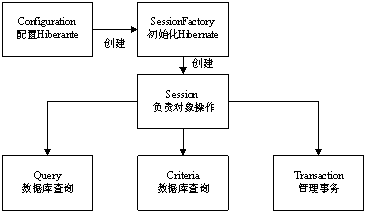
\includegraphics[width=11.1cm]{interface}
\caption{Hibernate核心接口}\label{fig:interface}
\vspace{\baselineskip}
\end{figure}

\section{AJAX技术}
AJAX[21]全称为“Asynchronous JavaScript and XML”(异步JavaScript和XML),是指一种创建交互式网页应用的网页开发技术。主要包含了以下几点技术:基于web标准(standards-based presentation)XHTML+CSS的表示;使用DOM(Document Object Model)进行动态显示及交互;使用XML和XSLT进行数据交换及相关操作;使用XMLHttpRequest进行异步数据查询、检索;使用JavaScript[22]将所有的东西绑定在一起。类似于DHTML或LAMP,AJAX不是指一种单一的技术,而是有机地利用了一系列相关的技术。使用Ajax的最大优点,就是能在不更新整个页面的前提下维护数据,这使得Web应用程序更为迅捷地回应用户动作,并避免了在网络上发送那些没有改变过的信息[23]。

\section{框架之间的有机整合}
Spring与Hibernate的集成是通过配置完成的。通过一个个的配置文件实现两者框架之间的连接。

Hibernate与Spring的集成。Spring 为持久层的开发提供了强有力的支持,其中对于Hibernate 的支持包括HibernateTemplate , HibernateInterceptor 和Hibernate transaction manager 。Hibernate 的连接、事务管理等是由SessionFactory 开始的,SessionFactory底层的DataSource 可以使用Spring 的IOC 注入,然后将SessionFactory 注入到相应的对象中。

% !Mode:: "TeX:UTF-8"

\chapter{研究工作总体安排与时间进度}
\begin{table}[!h]
\vspace{0.5em}\centering\xiaosi
\begin{tabular}{|c|c|c|}
\toprule[1.5pt]
任务序号 & 起止时间 & 阶段任务要点 \\
\midrule[1pt]
1 & 2010.11.30-2011.1.20 & \tabincell{c}{了解课题相关内容,查找中、\\英文资料} \\\hline
2 & 2011.1.21-2011.3.11 & \tabincell{c}{查阅文献资料,完成文献综述、\\开题报告和外文翻译} \\\hline
3 & 2011.3.12-2011.3.20 & \tabincell{c}{学习Spring、Hibernate、Ajax\\等开发相关技术} \\\hline
4 & 2011.3.21-2011.3.31 & 分析需求,确定开发工具 \\\hline
5 & 2011.4.1-2011.4.5 & 进行系统的概要设计 \\\hline
6 & 2011.4.6-2011.4.15 & 进行系统的详细设计 \\\hline
7 & 2011.4.16-2011.4.20 & 系统框架及开发环境搭建 \\\hline
8 & 2011.4.21-2011.5.21 & 进行项目的开发 \\\hline
9 & 2011.5.22-2011.5.25 & 完成系统测试 \\\hline
10 & 2011.5.26-2011.6.5 & 整理资料、完成毕业论文 \\\hline
11 & 2011.6.5-2009.6.10 & 上交毕业论文、准备毕业答辩 \\
\bottomrule[1.5pt]
\end{tabular}
\end{table}


\endgroup % 组结束
%%%%%%%%%% 参考文献 %%%%%%%%%%
\clearpage % 显式换页,使书签定位准确
\defaultfont
\bibliographystyle{GBT7714-2005NLang-ZJUT}
\phantomsection
\markboth{参考文献}{参考文献}
\addcontentsline{toc}{chapter}{参考文献}       % 参考文献加入到中文目录
\nocite{*}                                     % 若将此命令屏蔽掉,则未引用的文献不会出现在文后的参考文献中。
\bibliography{references/reference}

\end{document}
